\section{RQ3: Latency and energy at camera rates}
\label{sec:stream}

A backlog is the right workload for offline processing, but a camera
delivers frames at a fixed rate. We released the first 1,000 val2017
images at 15, 30 and 60\,fps and measured, for each frame, the time from
its release to its finished detection rows, together with module input
energy per frame (\cref{tab:stream,fig:stream}). The arrival-aware variant
(\cref{sec:pipelines}) is included here. On a backlog it reaches 194.8
images/s, 8.9\% less than the full pipeline (\cref{tab:ladder}).

\begin{table*}[t]
\centering
\caption{Streaming at fixed arrival rates (first 1,000 val2017 images, YOLO26n 640,
default governors, mean of two runs). Latency runs from frame arrival to finished
detection rows (ms). Energy is module input energy per frame (mJ). ``sat.'' marks a pipeline
that cannot sustain the arrival rate. Its queue grows without bound, so the
achieved rate is given instead of latency. $^\dagger$Near-saturated
cell: the achieved rate is 29.8\,images/s against 30\,fps arrivals in
both repeats, so the queue drains too slowly to clear between bursts
and p95 includes the resulting queuing. Idle input power alone is
312, 156 and 78\,mJ per frame at 15, 30 and 60\,fps.}
\label{tab:stream}
\small
\begin{tabular}{l rrr rrr rrr}
\toprule
& \multicolumn{3}{c}{15 fps} & \multicolumn{3}{c}{30 fps} & \multicolumn{3}{c}{60 fps} \\
\cmidrule(lr){2-4} \cmidrule(lr){5-7} \cmidrule(lr){8-10}
Pipeline & p50 & p95 & mJ & p50 & p95 & mJ & p50 & p95 & mJ \\
\midrule
Ultralytics & 32.0 & 38.4 & 357 & 36.2 & 188.0$^\dagger$ & 201 & \multicolumn{2}{c}{sat.\ (31/s)} & 194 \\
Float, sequential & 39.2 & 45.2 & 361 & 32.2 & 84.3 & 204 & \multicolumn{2}{c}{sat.\ (34/s)} & 187 \\
uint8, seq., event & 27.4 & 33.4 & 353 & 21.6 & 25.8 & 203 & \multicolumn{2}{c}{sat.\ (50/s)} & 151 \\
+ prefetch & 26.8 & 33.3 & 354 & 26.7 & 33.2 & 198 & 20.9 & 99.3 & 123 \\
+ overlap, 2 workers & 85.3 & 91.8 & 352 & 51.9 & 58.7 & 196 & 35.5 & 49.1 & 117 \\
+ arrival-aware overlap & 27.0 & 33.1 & 354 & 26.5 & 33.2 & 198 & 20.7 & 40.6 & 122 \\
\bottomrule
\end{tabular}
\end{table*}


\begin{figure}[t]
\centering
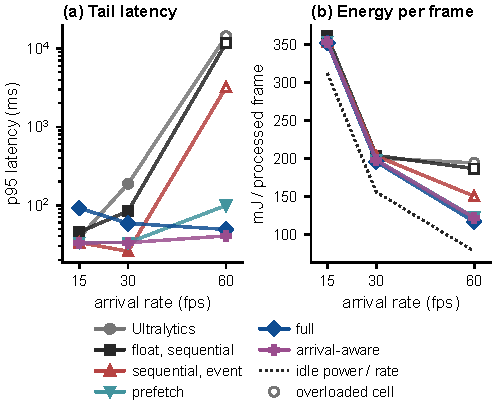
\includegraphics[width=\columnwidth]{figs/stream.pdf}
\caption{Streaming at 15, 30 and 60\,fps under default governors. Left:
p95 latency from frame release to finished rows (log scale); open
markers mark overloaded cells, where the processed rate falls short of
arrivals and the latency reflects a queue that grows over the finite
run, not a steady state.
Right: module input energy per \emph{processed} frame (the denominator
when a pipeline is overloaded); the dashed line is idle power divided by
the frame rate, the idle-reference contribution under the measured power state.}
\label{fig:stream}
\end{figure}

\textbf{Capacity.}
A pipeline that cannot sustain the arrival rate accumulates a queue,
and its latency grows with the run length. At 60\,fps this happens to
the Ultralytics predictor (31.0 images/s achieved), the float sequential
pipeline (34.2) and the uint8 sequential pipeline with event
synchronization (49.7); \cref{tab:stream} rounds these to whole images
per second. The Ultralytics predictor is also at the edge of its capacity at 30\,fps (29.8 images/s processed). Short stalls create queues that drain only slowly, and its latency distribution is strongly right-skewed (mean 55--64\,ms against medians of 36--37\,ms). An earlier harness version anchored the arrival clock before its own warm-up, which inflated exactly this tail (\cref{app:warmup}). Dropping the first 100 frames of every run moves the below-capacity p95 values by at most 4\,ms (188 to 192\,ms for the Ultralytics predictor at 30\,fps), so the remaining tails are steady-state queue drain, not start-up transients.
Capacity on a backlog therefore matters even for a camera application.
It is the margin that absorbs transient stalls.

\textbf{Energy is set by the idle floor.}
At 15\,fps every pipeline uses between 352 and 361\,mJ per frame. The
idle floor alone is 312\,mJ, or 86--89\% of the total. At 30\,fps the
spread is 196--204\,mJ against a floor of 156\,mJ. The full pipeline,
which uses 2.6$\times$ less energy per image than the Ultralytics
predictor on a backlog, uses only 2.5\% less at 30\,fps (195.7 versus
200.7\,mJ). Only at 60\,fps, where the slow pipelines saturate, does
the schedule decide energy again: 117--123\,mJ for the pipelines that
keep up, against 151--194\,mJ for those that do not, measured per
processed frame. This is the behavior described by \cref{eq:stream}. Using the idle power and the marginal energy measured on the backlog, \cref{eq:stream} with the arrival rate substituted agrees with every below-capacity streaming cell within $-0.2$ to $+11.6$\% (mean $+4.6$\%); the one slightly negative cell (Ultralytics at 15\,fps) lies inside the repeat spread of the backlog marginal estimate. For the three pipelines that saturate at 60\,fps the arrival-rate substitution underestimates by 10--37\%, because a queued pipeline never returns to the idle state the model assumes; substituting each pipeline's measured processed-frame rate instead (as the published aggregates do) brings the error on those cells to 0.3--0.5\%. The agreement below capacity comes mostly from the idle term, which dominates at camera rates. The marginal term alone is overestimated by 21--39\% for the uint8 pipelines running below capacity; for the two float-input pipelines it agrees within $-1.9$ to $+3.3$\%. The clock gap between the backlog and the stream does not explain the uint8 gap: the worst cell (the event-synchronized sequential pipeline at 15\,fps, $+39$\%) runs at 306\,MHz on both. The likely residue is CPU-side --- sleep and wake energy around each frame that the backlog marginal never pays. Whatever its origin, the backlog marginal energy is an empirical upper
envelope for the streaming marginal energy in every uint8 configuration we
measured, and is within 2--3\% of it for the float-input ones, not a prediction of it. At 15 and 30\,fps the GPU runs at about 306\,MHz in all
pipelines, so the marginal energy per frame is lower than on the
backlog, where the optimized pipelines run at about 1\,GHz. In this
regime the governor does what it is designed to do.

A corollary concerns clock locking. With \texttt{jetson\_clocks}, the
idle floor rises from 4.68 to 6.62\,W. At 30\,fps that is 221\,mJ per
frame before any work is done, already 8--13\% more than the total energy
of every default-governor pipeline in \cref{tab:stream}. For a camera
application below its capacity, locking clocks is an energy cost
without a throughput benefit.

\textbf{Latency is set by the schedule.}
At low rates the overlapped schedule has the worst latency of all
pipelines, despite having the highest backlog throughput. Its median
latency at 15\,fps is 85.3\,ms, against 27.4\,ms for the sequential
pipeline and 26.8\,ms for prefetch. Overlap finishes the rows of frame $i$ only
after frame $i{+}1$ has been decoded and enqueued, so every result
waits about one inter-arrival period (66.7\,ms at 15\,fps). The penalty
shrinks as the rate grows (51.9\,ms at 30\,fps, 35.5\,ms at 60\,fps).
The sequential pipeline is the fastest per frame at 30\,fps (median 21.6,
p95 25.8\,ms), and it keeps up with margin to spare (its backlog
capacity of ${\approx}50$\,images/s exceeds the 30\,fps arrival rate by
two thirds), but at 60\,fps it fails.
Plain prefetch keeps up at 60\,fps, but its p95 rises to 99.3\,ms. At
60\,fps the governor runs prefetch at about 410\,MHz, so its margin
over the arrival rate is small and transient stalls build queues.

The arrival-aware variant combines the two behaviors. When the next
frame is not yet available, it finishes the in-flight frame instead of
holding it. When frames queue up, it overlaps as before. Its p95 latency is within 7.4\,ms of the best pipeline at every rate (p95 33.1, 33.2 and 40.6\,ms at
15, 30 and 60\,fps), it is the only pipeline whose p95 stays at or below
41\,ms at all three rates, and its energy is within 0.4--4.3\% of the
full pipeline. Its predictions are byte-identical to the other uint8
pipelines.

The latency of the sequential pipeline also depends on the CPU
governor. Its median falls from 27.4\,ms at 15\,fps to 21.6\,ms at
30\,fps, although the work per frame is the same. At the lower rate the
CPU is idle for longer between frames, and its CPU time per frame rises
from 23.5\,ms at 30\,fps to 29.4\,ms at 15\,fps. This is
consistent with \cref{sec:sched}'s backlog finding ---
\texttt{schedutil} lowers the clock while the waiting thread sleeps
--- but we did not log the CPU clock in the streaming runs, so we
offer it as a plausible mechanism rather than a demonstrated one.

\textbf{Answer to RQ3.}
At camera rates below a pipeline's capacity, energy per frame is
dominated by the idle floor. The pipelines we tested differ by at most 2.5\% at 15\,fps and 4.2\% at 30\,fps. The schedule mainly determines
latency and capacity margin. The schedule with the best backlog
throughput has the worst latency at 15\,fps, because it holds every
result for one frame period. An arrival-aware schedule removes this
penalty at a cost of 8.9\% of backlog throughput and at most 4.3\% of
energy. Locking clocks raises the idle floor and is counterproductive
in this regime.
